\documentclass[letterpaper,11pt]{article}

\usepackage{listings}
\usepackage{color}

\definecolor{dkgreen}{rgb}{0,0.6,0}
\definecolor{gray}{rgb}{0.5,0.5,0.5}
\definecolor{mauve}{rgb}{0.58,0,0.82}

\lstset{frame=tb,
  language=Python,
  aboveskip=3mm,
  belowskip=3mm,
  showstringspaces=false,
  columns=flexible,
  basicstyle={\small\ttfamily},
  numbers=none,
  numberstyle=\tiny\color{gray},
  keywordstyle=\color{blue},
  commentstyle=\color{dkgreen},
  stringstyle=\color{mauve},
  breaklines=true,
  breakatwhitespace=true,
  tabsize=3
}

\usepackage{setspace}
\usepackage{graphicx}
\usepackage{indentfirst}
\usepackage{bm}    %for textbf
\usepackage{amsmath}
\usepackage{amsfonts}   %for mathbb
\allowdisplaybreaks[4]  %from {amsmath}
\newcommand{\independent}{\rotatebox[origin=c]{90}{$\models$}}  %from {graphicx}
\usepackage{geometry}
\geometry{letterpaper, scale=0.8}  %from {geometry}
\author{Yuan Yin A20447290}
\title{MATH 588 Homework 2}
\begin{document}\large
\maketitle
\begin{spacing}{1.2}  %from {setspace}
\section*{Problem 1}

\textbf{Value at Risk}

Pros: First the definition is easy to understand. It looks directly related to risk. Also easy to compute, and have nice properties like monotonicity and homogeneity. It's convenient to compare VaR between assets.

Cons: Like said on class, it doesn't make sence in some cases. Since it's not subadditive for some cases. Besides, it only shows the quantile but not clearify what really happens beyond this significance level(i.e. what the worst case could be). Also, when a portfolio has many assets. The cost to compute VaR grows fast. Also, VaR is only easy to compute when there are simple assumptions like Gaussian or t distribution, which is not realistic.

\section*{Problem 2}

Prove the properties:

1. For continuous r.v.s the cdf F is $\uparrow$, while for discrete r.v.s F is $\nearrow$ with some flat parts.

\textbf{Proof:} For continuous r.v. X, the pdf $f(x)$ is also continuous and positive on domain. Thus the cdf $F(x) = \int_{-\infty}^x f(t)dt$ is a strictly increasing function.

For discrete r.v. Y, the cdf is represented as $F(y) = \sum_{y_i \le y} \mathbb{P}(Y=y_i)$. Thus when $y \in [y_i, y_{i+1}) 
\  \forall i$, the cdf $F(y)$ is flat, otherwise, it's increasing.

2. $x_0 = VaR_{\alpha}(L)$ iff $F_L(x_0) \ge \alpha$ and $F_L(x) < \alpha$ for all $x < x_0$.

\textbf{Proof:} ``$\Rightarrow$'' By definition, $VaR_{\alpha}(L) = \inf \{l \in \mathbb{R} | F_L(l) \ge \alpha\}$. Thus $F_L(x_0) \ge \alpha$ and $F_L(x) < \alpha$ for all $x < x_0$.

``$\Leftarrow$'' Since $F_L(x_0) \ge \alpha$, by definition of VaR, $x_0 \ge VaR_{\alpha}(L)$. Besides, $F_L(x) < \alpha$ for all $x < x_0$, thus $x_0 = \inf \{l \in \mathbb{R} | F_L(l) \ge \alpha\}$. By definition, $x_0 = VaR_{\alpha}(L)$.

3. If $F_L$ is $\uparrow$, then there exists unique $x_0$ such that $F_L(x_0) = \alpha$ and $x_0 = VaR_\alpha(L)$.

\textbf{Proof:} From property 1, we get the random variable L is a continuous r.v.(since strictly increasing). Then, the cdf $F_L$ is also continuous function. Thus, there exists as least one $x_0$ such that $F_L(x_0) = \alpha, \ \alpha \in (0,1)$. For uniqueness, since $F_L$ is strictly increasing, for $\forall \epsilon > 0$ (small enough), $F_L(x_0+\epsilon) > F_L(x_0)$ and $F_L(x_0-\epsilon) < F_L(x_0)$. Thus by definition of VaR, $x_0 = VaR_{\alpha}(L)$.

4. If $L \le 0$, then $VaR_{\alpha}(L) \le 0$.

\textbf{Proof:} By definition, $VaR_{\alpha}(L) = \inf \{l \in \mathbb{R} | F_L(l) \ge \alpha\}$. Since $L \le 0 \Rightarrow l \le 0$. Thus, $VaR_{\alpha}(L) \le 0$

5. (monotonicity) If $L^1 \le L^2$, then $VaR_{\alpha}(L^1) \le VaR_{\alpha} (L^2)$.

\textbf{Proof:} $L^1(\omega) \le L^2(\omega), \ \forall \omega \in \Omega$. Therefore, $\{L^1(\omega) \le l\} \supseteq \{L^2(\omega) \le l\} \Rightarrow \mathbb{P}\{L^1(\omega) \le l\} \ge \mathbb{P}\{L^2(\omega) \le l\}$. Thus for $\forall \alpha \in \mathbb{R}$, $\mathbb{P}\{L^1(\omega) \le l\} \ge \alpha \Rightarrow \mathbb{P}\{L^2(\omega) \le l\} \ge \alpha$, i.e. $\{l: \mathbb{P}\{L^1(\omega) \le l\} \ge \alpha\} \subseteq \{l: \mathbb{P}\{L^2(\omega) \le l\} \ge \alpha\}$. Take inf on both sides, and we get $VaR_{\alpha}(L^1) \le VaR_{\alpha} (L^2)$ by definition.

6. (homogeneity) $VaR_{\alpha}(\lambda L) = \lambda VaR_{\alpha}(L)$, for any $\lambda \ge 0$.

\textbf{Proof:}

\begin{equation}
\begin{aligned}
VaR_{\alpha}(\lambda L) &= \inf \{l \in \mathbb{R} | \mathbb{P}(\lambda L \le l) \ge \alpha\} \\
&= \inf \{l \in \mathbb{R} | \mathbb{P}(L \le l/\lambda) \ge \alpha\} \\
&= \inf \{\frac{l}{\lambda} \lambda \in \mathbb{R} | \mathbb{P}(L \le l/\lambda) \ge \alpha\} \\
&= \lambda \inf \{\frac{l}{\lambda} \in \mathbb{R} | \mathbb{P}(L \le l/\lambda) \ge \alpha\} \\
&= \lambda VaR_{\alpha}(L)
\end{aligned}
\end{equation}

7. (cash-additive) $VaR_{\alpha}(L+m) = VaR_{\alpha}(L) + m$, for any $m \in \mathbb{R}$.

\textbf{Proof:} Similar to property 6,

\begin{equation}
\begin{aligned}
VaR_{\alpha}(L + m) &= \inf \{l \in \mathbb{R} | \mathbb{P}(L + m \le l) \ge \alpha\} \\
&= \inf \{l \in \mathbb{R} | \mathbb{P}(L \le l - m) \ge \alpha\} \\
&= \inf \{l - m + m \in \mathbb{R} | \mathbb{P}(L \le l - m) \ge \alpha\} \\
&= m + \inf \{l - m \in \mathbb{R} | \mathbb{P}(L \le l - m) \ge \alpha\} \\
&= m + VaR_{\alpha}(L)
\end{aligned}
\end{equation}

8. $VaR_{\alpha}(L - VaR_{\alpha}(L)) = 0$, fair capital reserve.

\textbf{Proof:} Suppose $m = - VaR_{\alpha}(L)$ and use property 7 by replacing m, then get the result.

\section*{Problem 3}

If there is $L_1,\ldots, L_n$ which all indepent and has distribution with $L$ in slide 13. Then the possible loss:

\begin{center}
\begin{tabular}{|c|c|}
\hline
$L^1+L^2+\ldots+L^n$&$-50(n-i)+1000(n)$\\
\hline
$\mathbb{P}$&$\dbinom{n}{i} (1-p)^{n-i}p^i$\\
\hline
\end{tabular}
\end{center}

where $i = 1, 2, \ldots, n$.

Now we assume $p=0.009$ and take $\alpha = 0.99$. Then $VaR_{\alpha}(L^i) = -50$ and therefore $VaR_{\alpha}(L^1)+\ldots+VaR_{\alpha}(L^n) = -50n$.

However, $L^1+\ldots+L^n \le -50n$ if and only if $i=0$, i.e. all $L^i = -50$. And thus $\mathbb{P}(L^1+\ldots+L^n \le -50n) = (1-p)^n = 0.991^n < 0.99 = \alpha$.

Since by definition of value-at-risk,$VaR_{\alpha}(L) = \inf \{l|\mathbb{P}(L \le l) \ge \alpha\}$, thus $\alpha \le \mathbb{P}(L^1+\ldots+L^n \le VaR_{\alpha}(L^1+\ldots+L^n))$.

From two inquality above, we can get $\mathbb{P}(L^1+\ldots+L^n \le -50n) \le \mathbb{P}(L^1+\ldots+L^n \le VaR_{\alpha}(L^1+\ldots+L^n))$. And thus: $\Rightarrow VaR_{\alpha}(L^1+\ldots+L^n) \ge -50n = VaR_{\alpha}(L^1)+\ldots+VaR_{\alpha}(L^n)$

We can conclude that this example is still superadditive.

\section*{Problem 4}
Suppose $t_{\nu}$ is the cdf of standard $t_{\nu}$ distribution and $g_{\nu}$ is the corresponding pdf.

Since L is continuous

\begin{equation}
\begin{aligned}
ES_{\alpha}(L) &=\mathbb{E}[\mu+\sigma t_{\nu} | \frac{L-\mu}{\sigma} \ge \frac{VaR_{\alpha}(L) - \mu}{\sigma}] \\
&= \mu + \sigma \mathbb{E}[t_{\nu} | t_{\nu} \ge VaR_{\alpha} (\frac{L-\mu}{\sigma})] \quad \text{homogenity and cash-additive} \\
&= \mu + \sigma ES_{\alpha}(t_{\nu})
\end{aligned}
\end{equation}

Besides,

\begin{equation}
\begin{aligned}
ES_{\alpha}(t_{\nu}) &= \frac{1}{1-\alpha} \int_{t_{\nu}^{-1}(\alpha)}^{\infty} tg_{\nu}(t) dt \\
&= \frac{1}{1-\alpha} \int_{t_{\nu}^{-1}(\alpha)}^{\infty} a(1+\frac{t^2}{\nu})^{-\frac{\nu+1}{2}}t dt \\
\end{aligned}
\end{equation}

where $a:= \frac{\Gamma(\frac{\nu + 1}{2})}{\sqrt{\nu \pi} \Gamma(\frac{\nu}{2})}$.

Now assume $z = t^2$ and replace all t above, we get:

\begin{equation}
\begin{aligned}
ES_{\alpha}(t_{\nu}) &= \frac{1}{1-\alpha} \int_{(t_{\nu}^{-1}(\alpha))^2}^{\infty} \frac{a}{2} (1+\frac{z}{\nu})^{-\frac{\nu+1}{2}} dz \\
&= \frac{1}{1-\alpha} \int_{(t_{\nu}^{-1}(\alpha))^2}^{\infty} \frac{a}{2} \frac{\nu}{-\frac{\nu+1}{2}+1} d((1+\frac{z}{\nu})^{-\frac{\nu+1}{2}+1}) \\
&= \frac{1}{1-\alpha} \frac{a\nu}{1-\nu} [(1+\frac{z}{\nu})^{-\frac{\nu+1}{2}+1}] \Bigg|_{(t_{\nu}^{-1}(\alpha))^2}^{\infty} \\
&= \frac{a\nu}{(1-\alpha)(\nu-1)} (1+\frac{(t_{\nu}^{-1}(\alpha))^2}{\nu})^{-\frac{\nu+1}{2}+1} \\
&= \frac{a}{(1-\alpha)(\nu-1)} (1+\frac{(t_{\nu}^{-1}(\alpha))^2}{\nu})^{-\frac{\nu+1}{2}} \cdot (1+\frac{(t_{\nu}^{-1}(\alpha))^2}{\nu})\cdot \nu  \\
&= \frac{1}{(1-\alpha)(\nu-1)} g_{\nu}(t_{\nu}^{-1}(\alpha)) \cdot (\nu+(t_{\nu}^{-1}(\alpha))^2) \\
&= \frac{g_{\nu}(t_{\nu}^{-1}(\alpha))}{1-\alpha} \cdot \frac{\nu+(t_{\nu}^{-1}(\alpha))^2}{\nu-1}
\end{aligned}
\end{equation}

Here we require $\nu > 1$.

Thus we get 

$$
ES_{\alpha}(L) = \mu + \sigma \cdot \frac{g_{\nu}(t_{\nu}^{-1}(\alpha))}{1-\alpha} \cdot \frac{\nu+(t_{\nu}^{-1}(\alpha))^2}{\nu-1}
$$

\section*{Problem 5}
The distribution of the sum of two independent exponential is gamma distribution (here I mean $L^1+L^2$). And I solve this problem in a numerical method by varying $\lambda$. Thus, $VaR_{\alpha}(L^1+L^2)$ is the quantile for $Gamma(2,\lambda)$ distribution at $\alpha$. And $VaR_{\alpha}(L^1)+VaR_{\alpha}(L^2) = 2*VaR_{\alpha}(L^1)$ is twice of quantile of $Exp(\lambda)$ distribution at $\alpha$. I compute the both $VaR_{0.99}(L_1+L_2)$ and $VaR_{0.99}(L_1)+VaR_{0.99}(L_2)$.


First, I plot when varying $\lambda$ from 0 to 2, the value-at-risk for both:

\begin{figure}[t]        
 \center{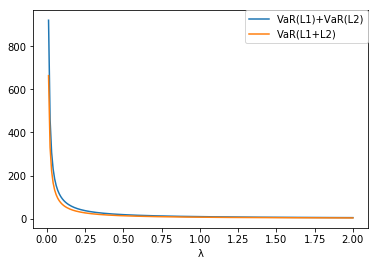
\includegraphics[scale=0.5]  {problem5(1).png}}        
 \caption{\label{1} Comparing two equation}      
 \end{figure}

Then I plot the difference:
$$\Delta = VaR_{0.99}(L^1+L^2) - (VaR_{0.99}(L^1)+VaR_{0.99}(L^2))$$

\begin{figure}[t]        
 \center{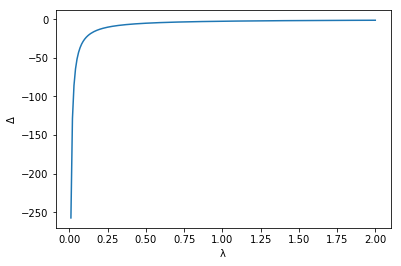
\includegraphics[scale=0.5]  {problem5(2).png}}        
 \caption{\label{1} The function of difference}      
 \end{figure}

Since we want to find supperadditive, which means we want to find interval of $\lambda$ such that the function is above $0$. However, as the plot below, we can see that there is no such interval, all values are below zero and getting close to zero when $\lambda$ increases.



\section*{Bonus}

Prove the properties of ES:

1,2 and 3 have no relation to ES. We start from 4:

4. If $L \le 0$, then $ES_{\alpha}(L) \le 0$.

\textbf{Proof:} By definition, $ES_{\alpha}(L) = \frac{1}{1-\alpha} \int_{\alpha}^1 VaR_{\beta}(L) d\beta$. Since $L \le 0 \Rightarrow VaR_{\beta}(L) \le 0$ from porperty 4 of VaR, $\alpha \in (0,1) \Rightarrow \frac{1}{1-\alpha} > 0$. Thus, $ES_{\alpha}(L) \le 0$

5. (monotonicity) If $L^1 \le L^2$, then $ES_{\alpha}(L^1) \le ES_{\alpha} (L^2)$.

\textbf{Proof:} Since by property 5 of VaR, $L^1 \le L^2 \Rightarrow VaR_{\alpha}(L^1) \le VaR_{\alpha} (L^2)$. By definition, $\frac{1}{1-\alpha} \int_{\alpha}^1 VaR_{\beta}(L_1) d\beta \le \frac{1}{1-\alpha} \int_{\alpha}^1 VaR_{\beta}(L_2) d\beta$, where $\alpha \in (0,1) \Rightarrow \frac{1}{1-\alpha} > 0$.

6. (homogeneity) $ES_{\alpha}(\lambda L) = \lambda ES_{\alpha}(L)$, for any $\lambda \ge 0$.

\textbf{Proof:} Again, we use property 6 of VaR:

\begin{equation}
\begin{aligned}
ES_{\alpha}(\lambda L) &= \frac{1}{1-\alpha} \int_{\alpha}^1 VaR_{\beta}(\lambda L) d\beta \\
&= \frac{1}{1-\alpha} \int_{\alpha}^1 \lambda VaR_{\beta}(L) d\beta \\
&= \lambda \frac{1}{1-\alpha} \int_{\alpha}^1 VaR_{\beta}(L) d\beta \\
&= \lambda ES_{\alpha}(\lambda L)
\end{aligned}
\end{equation}

7. (cash-additive) $ES_{\alpha}(L+m) = ES_{\alpha}(L) + m$, for any $m \in \mathbb{R}$.

\textbf{Proof:} Similar to property 5,

\begin{equation}
\begin{aligned}
ES_{\alpha}(L + m) &= \frac{1}{1-\alpha} \int_{\alpha}^1 VaR_{\beta}(L+m) d\beta \\
&= \frac{1}{1-\alpha} \int_{\alpha}^1 (VaR_{\beta}(L) + m) d\beta \\
&= \frac{1}{1-\alpha} \int_{\alpha}^1 VaR_{\beta}(L) d\beta + \frac{1}{1-\alpha} \int_{\alpha}^1 m d\beta \\
&= ES_{\alpha}(L) + m
\end{aligned}
\end{equation}

8. $ES_{\alpha}(L - ES_{\alpha}(L)) = 0$, fair capital reserve.

\textbf{Proof:} Suppose $m = - ES_{\alpha}(L)$ and use property 7 by replacing m, then get the result.

\section*{Appendix}
\textbf{code for problem 5:}
\begin{lstlisting}[title=code for problem 5, frame=shadowbox]
alpha = 0.99
lambda_ = [(i+1)*0.01 for i in range(200)]
VaR_gamma = []
VaR_expon = []
for lam in lambda_:
    VaR_expon.append(2*expon.ppf(alpha, scale=1/lam))
    VaR_gamma.append(gamma.ppf(alpha, a=2, scale=1/lam))

VaR_expon = np.array(VaR_expon)
VaR_gamma = np.array(VaR_gamma)


plt.xlabel('\u03BB')
#plt.ylabel('\u0394')
#plt.plot(lambda_, np.array([VaR_expon, VaR_gamma]).T)
plt.plot(lambda_, VaR_expon.T,label="VaR(L1)+VaR(L2)")
plt.plot(lambda_, VaR_gamma.T,label="VaR(L1+L2)")

plt.legend(bbox_to_anchor=(1.0, 1), loc=1, borderaxespad=0.)

#plt.plot(lambda_, (VaR_gamma - VaR_expon).T)
plt.show()
\end{lstlisting}

\end{spacing}
\end{document}